\section{Results}
\label{sec:results}

All 139 requests to \gpt\ produced a valid circuit or weight vector on the first attempt; the repair loop was never used. Full per-condition tables are in Appendix~\ref{app:tables}; this section walks through the three families.

\subsection{VQE: the model writes ground-state parameters}

\begin{figure}[tbp]
\centering
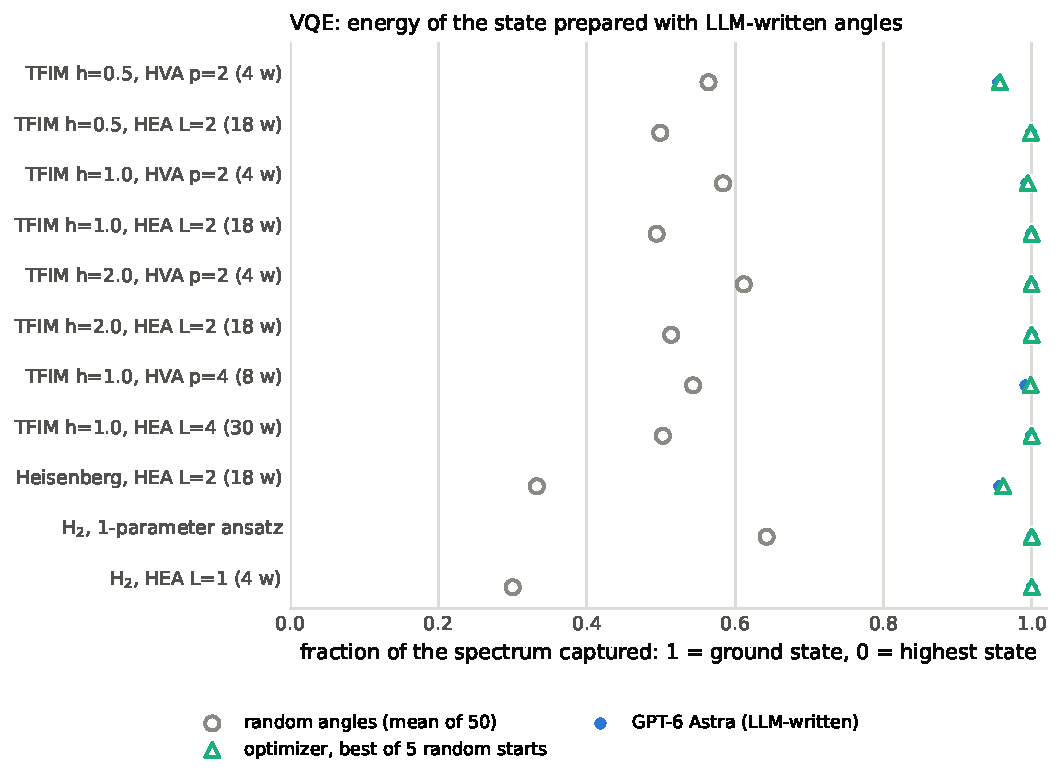
\includegraphics[width=0.9\linewidth]{figures/vqe.pdf}
\caption{VQE. Fraction of the spectrum captured by the state prepared with the model's angles ($1$ = exact ground state), mean $\pm$ s.d.\ over three requests, against random angles and an optimizer with five random restarts on the same circuit.}
\label{fig:vqe}
\end{figure}

Figure~\ref{fig:vqe} and Table~\ref{tab:vqe_full} summarize eleven problem--ansatz pairs. On every one the model's angles are within $0.007$ of the optimizer on the $[0, 1]$ spectrum scale, and on seven of eleven they are within $0.001$. Random angles sit at $0.30$--$0.64$.

For the transverse-field Ising chain with the Hamiltonian variational ansatz (four angles) the model reaches $0.955$, $0.993$ and $1.000$ at $h = 0.5, 1, 2$, against an optimizer ceiling of $0.957$, $0.995$ and $1.000$: the ansatz itself is the limit, and the model finds its optimum. Its angles move with the field the way the physics says they should: the coupling angle of the first layer falls from $0.55$ to $0.47$ to $0.24$ as $h$ grows from $0.5$ to $2$, while the field angle rises from $1.20$ to $1.36$, and the three repeats of each problem agree to within $0.1$ rad. With the 18-angle hardware-efficient ansatz the model reaches $0.999$--$1.000$ on all three fields; its replies describe the target state (``a ferromagnetic state with modest canting toward $+X$, strongest at the boundaries'') and set the angles to produce it. For the critical chain with a 30-angle HEA it still reaches $0.999$, by setting 19--21 of the 30 angles to exactly zero and programming one rotation layer plus one correction layer; with the eight-angle HVA it reaches $0.992$ against $0.999$ for the optimizer, the one case where more angles made the model slightly worse rather than better.

For H$_2$ the model does something different: it derives the energy as a function of the single angle, $E(\theta) = -1.0520 - 0.7782\cos\theta + 0.1820\sin\theta$ (which is correct for the stated Hamiltonian and circuit), and returns its minimizer $\theta^\ast = -\arctan(0.1820/0.7782) = -0.2297$, the exact ground state. With the four-angle HEA on the same molecule it also reaches the exact energy. The largest gaps are the eight-angle HVA ($0.007$) and the Heisenberg chain with the HEA ($0.956$ vs $0.962$); on the latter its reply reasons about singlet pairing on bonds but the real-amplitude HEA cannot represent the singlet ground state well with two layers, and both model and optimizer are limited by it.

\subsection{QAOA: the model writes angle schedules}

\begin{figure}[tbp]
\centering
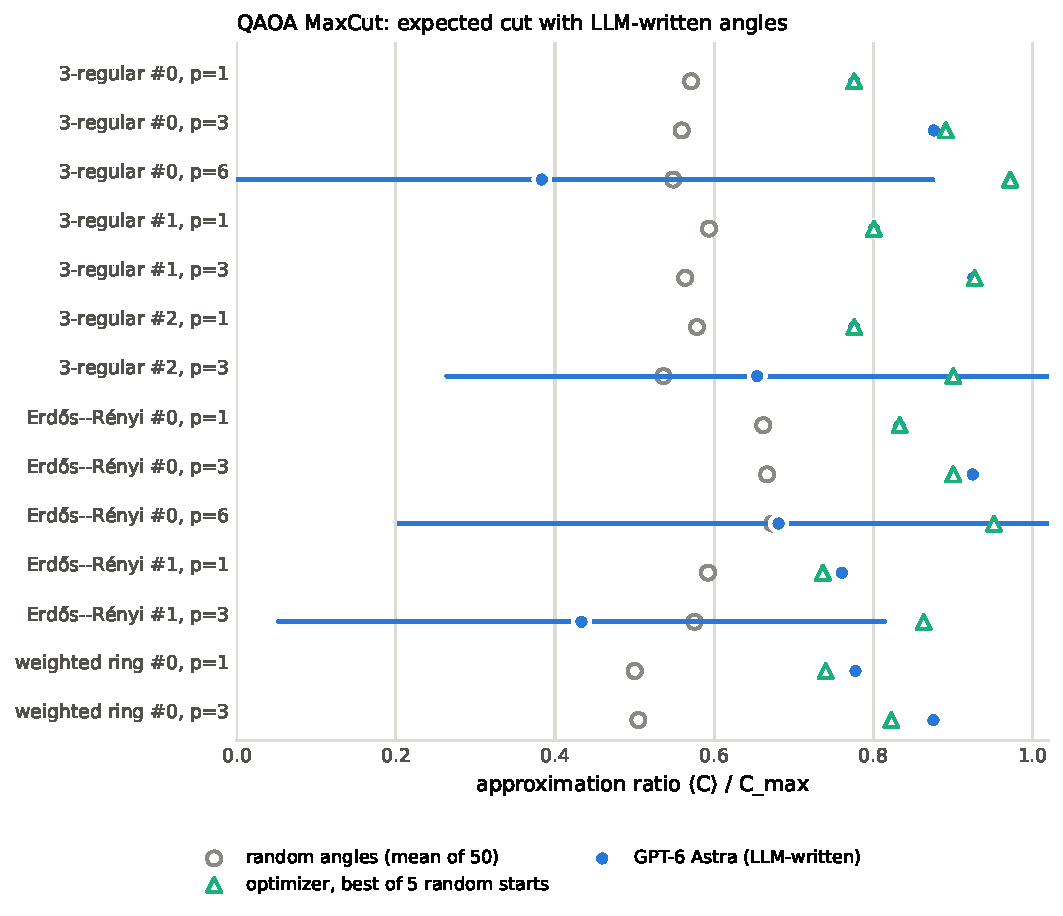
\includegraphics[width=0.9\linewidth]{figures/qaoa.pdf}
\caption{QAOA MaxCut on eight-node graphs. Approximation ratio $\langle C\rangle / C_{\max}$ with the model's angles, against random angles and an optimizer with five random restarts. The large spreads at $p = 3$ and $p = 6$ are sign errors on the mixing angles in 6 of 42 requests (see text).}
\label{fig:qaoa}
\end{figure}

At depth $p = 1$ the model's angles are optimal on all six graphs ($0.776$, $0.801$, $0.776$, $0.833$, $0.760$, $0.778$, with zero variance across repeats): in every one of the 18 requests they reach the best value the optimizer found on that graph, and on the second Erd\H{o}s--R\'enyi graph and the weighted ring the five-restart optimizer itself fell short of that value in one run of three (mean $0.737$ and $0.740$), so the model's average is above the optimizer's. Its method is analytic: for the first 3-regular graph it writes ``the exact $p = 1$ expectation is $6 + 6\sin(4\beta)\sin(\gamma)\cos^2(\gamma) - 6\sin^2(2\beta)\sin^2(\gamma)\cos^2(\gamma)$'', accounting for the graph's four triangles, and maximizes it in closed form. At $p = 3$ and $p = 6$ it writes a smooth schedule---cost angles increasing, mixing angles decreasing across layers, a pattern known from the literature on parameter concentration---and where the schedule has the right sign it is within $0.03$ of the optimizer or above it ($0.925$ vs $0.901$ on the first Erd\H{o}s--R\'enyi graph at $p = 3$, $0.876$ vs $0.823$ on the weighted ring).

Six of the 42 requests failed in one specific way: every mixing angle was negated (\eg\ $[0.38, -0.57, 0.65, -0.47, \ldots]$ instead of $[0.36, 0.57, 0.62, 0.47, \ldots]$). Negating $\beta$ alone is not a symmetry of QAOA, and those circuits score $0.10$--$0.22$. Re-evaluating them with $|\beta|$ gives $0.87$--$0.96$, at the optimizer's level in every case. Over all 42 requests the mean ratio is $0.748$ as written and $0.856$ with the sign corrected, against $0.849$ for the optimizer; over the 36 sign-correct requests it is $0.846$ against $0.838$. We report the as-written number as the result and the corrected one as the diagnosis.

\subsection{Warm starts}

\begin{figure}[tbp]
\centering
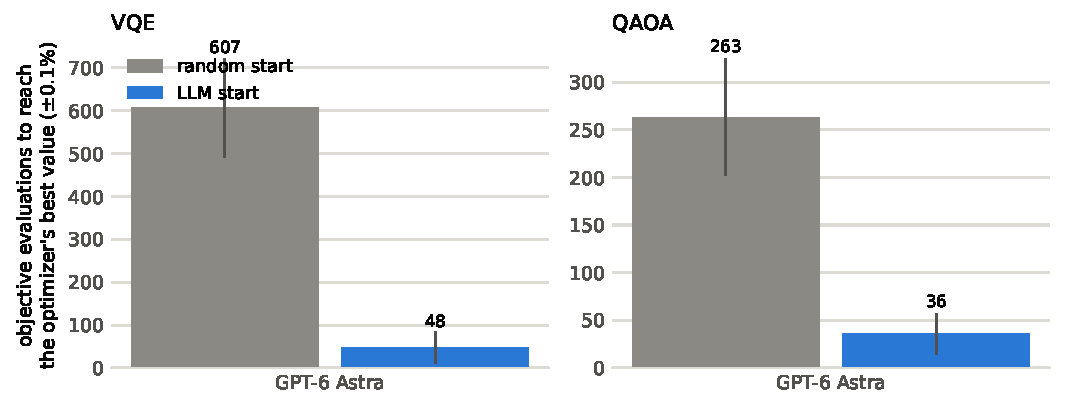
\includegraphics[width=0.85\linewidth]{figures/warmstart.pdf}
\caption{Loss evaluations the optimizer needs to come within $0.1\%$ of the best value found from random starts, when started from random angles versus from the model's angles (mean $\pm$ s.e.\ over all VQE and QAOA requests).}
\label{fig:warmstart}
\end{figure}

Started from the model's angles, L-BFGS-B reached the target in a median of one loss evaluation in both VQE and QAOA, meaning the model's point was already within tolerance in 61\% (VQE) and 64\% (QAOA) of requests; the means are $48$ and $36$ evaluations, against $607$ and $263$ from random starts (Figure~\ref{fig:warmstart}). The warm start also succeeds more often: it reached the target in $91\%$ of VQE and $93\%$ of QAOA runs, against $81\%$ and $46\%$ for random starts. The failures to reach it from the model's angles are the sign-flipped QAOA schedules and the Heisenberg chain, where the optimizer from the model's point converges to a slightly different local minimum.

\subsection{QML: writing a classifier's weights}

\begin{figure}[tbp]
\centering
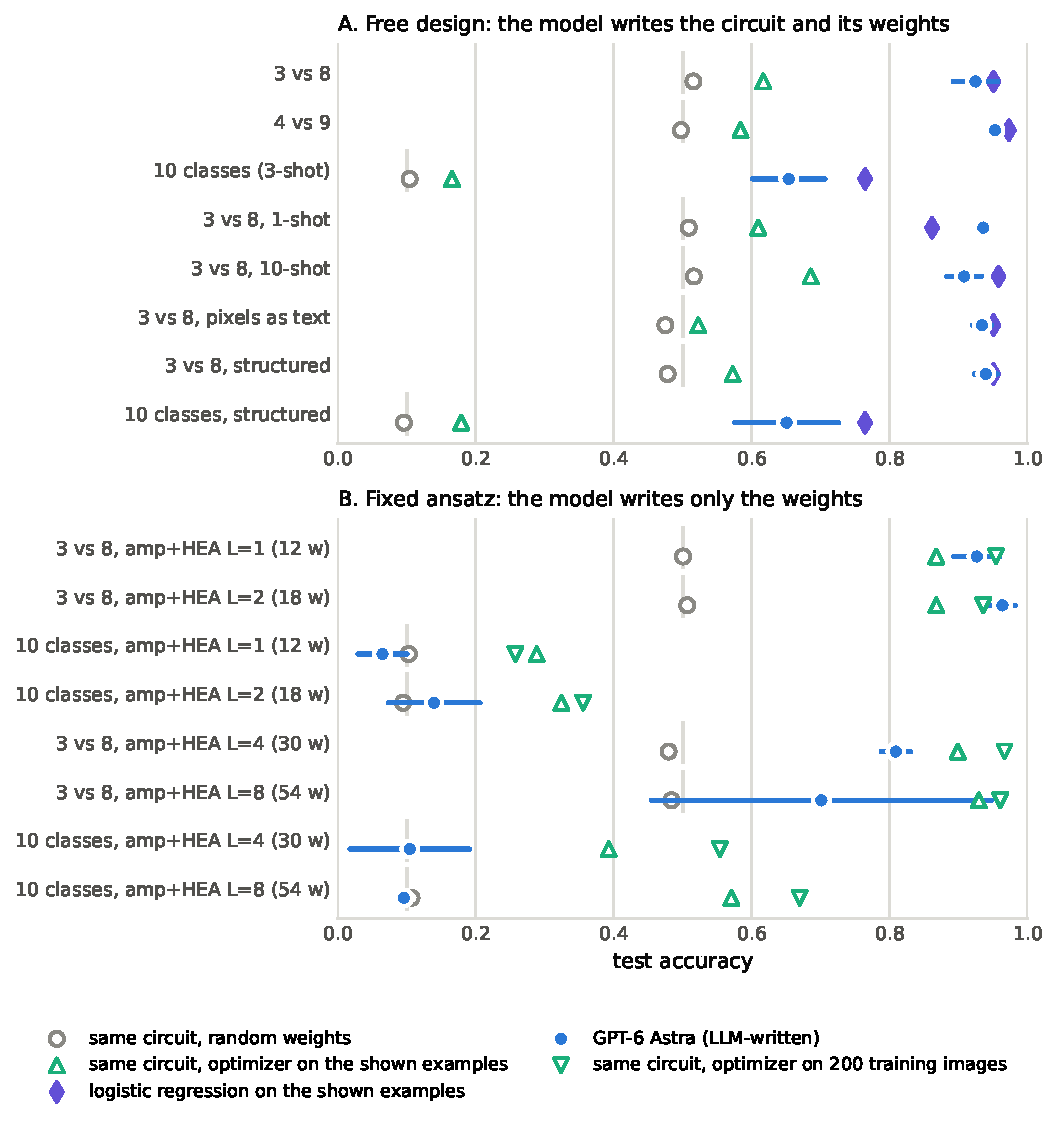
\includegraphics[width=0.9\linewidth]{figures/qml.pdf}
\caption{Digit classification. Test accuracy of the model's circuit (mean $\pm$ s.d.\ over five requests in A, three in B), with the same circuit under random weights, under an optimizer that saw the same examples, and logistic regression on those examples (A) or the optimizer with 200 training images (B). Gray ticks mark chance.}
\label{fig:qml}
\end{figure}

\paragraph{Free design.}
Given five examples per class and a circuit language, the model's circuits score $0.924 \pm 0.032$ on 3 vs 8 and $0.952 \pm 0.008$ on 4 vs 9 (chance $0.5$), against $0.50$ with random weights on the same circuits and $0.58$--$0.62$ for an optimizer that trained the same circuits on the same ten examples (Figure~\ref{fig:qml}A, Table~\ref{tab:qml_free_full}). Logistic regression on the ten examples scores $0.95$--$0.97$. The number of examples barely matters: with one example per class the model scores $0.935$, with ten $0.907$, and shown the pixel grids as integers instead of images $0.933$. On all ten classes with three examples each it scores $0.653 \pm 0.053$ (chance $0.1$), against $0.17$ for the optimizer on the same thirty images and $0.76$ for logistic regression.

In all 30 unconstrained requests the model designed the same kind of circuit: chains of $ry$ rotations each driven by one pixel (plus a bias rotation), with a bit-string readout. In all 25 binary requests the circuit is a single qubit carrying one such chain of 8--51 rotations. As explained in Section~\ref{sec:discussion}, this is a linear classifier with a smooth threshold, and the model's replies describe it as one (``positive weights collect middle-left evidence, and negative weights compensate for right-side ink''). For ten classes it scaled the same idea up: six to eight qubits, each a rotation chain detecting one feature (``central versus peripheral ink, upper and lower stroke balance, crossbars, and bottom closure''), read out compositionally so that, in its words, ``5 combines a left-upper-stroke detector with lower-right dominance''. Three of the five ten-class circuits went further and used controlled-$ry$ gates, two of them with Toffoli gates as well, to implement that logic explicitly, scoring $0.67$--$0.71$. Fine-tuning the model's weights with the optimizer on the shown examples did not help on any binary task ($0.85$--$0.95$ after versus $0.91$--$0.95$ before): the optimizer, with ten examples, overfits where the model's prior does not.

\paragraph{Structured design.}
With the three structural rules (at least two qubits, at least one two-qubit gate, no consecutive same-axis rotations on a qubit) the model scores $0.939 \pm 0.015$ on 3 vs 8 and $0.650 \pm 0.067$ on ten classes, indistinguishable from the unconstrained $0.924$ and $0.653$, and all ten circuits are valid on the first attempt. What it built is the more interesting result. In every binary trial the model kept the linear accumulator and found a circuit identity that satisfies the rules: it interleaves $z$ gates between the $ry$ rotations (since $z\,ry(b)\,z = ry(-b)$, the chain still sums, with alternating signs absorbed into the weights; ``alternating Z gates and signed RY angles accumulate this evidence into one decision angle'', it explains), or accumulates the same weighted sum as a phase with $p$ or $rz$ gates between CNOTs and converts it to a probability with a final Hadamard, and then moves the result to the readout qubit with a single CNOT. For ten classes two of the five circuits are of the same kind (``the $\pi$-angle ZZ gates provide sign refocusing between successive encoding rotations''), and three use genuinely multi-qubit designs: 117 $u3$ rotations with 12 CNOTs on five qubits ($0.706$), and two eight-qubit circuits in which ``four address qubits select a class-specific affine phase; interference converts that phase into a score monotonic in a sparse nearest-prototype discriminant'', built from 39 Toffoli and 146 controlled-phase gates ($0.713$, the best ten-class circuit of the study). The model, in other words, knows exactly which weight space it wants to program---a signed sum of pixels---and, forbidden the obvious circuit for it, writes a different circuit that computes the same thing, or, when it must, a nearest-prototype classifier whose prototypes it writes by hand.


\paragraph{Fixed ansatz and scaling.}
When the circuit is fixed to amplitude encoding of the whole image followed by a hardware-efficient ansatz, the model has no interpretable pixel weights to write; it must reason about how rotations on the row and column qubits redistribute amplitude. For 3 vs 8 with 12 and 18 weights it does this well: $0.926 \pm 0.033$ and $0.963 \pm 0.019$, above the optimizer trained on the same examples ($0.867$) and close to the optimizer with 200 images ($0.935$--$0.954$). Its reply reads the circuit correctly (``3 has more ink energy in the outer row bands relative to the middle bands, while 8 is more centrally distributed; these angles implement that row-band contrast'').

\begin{figure}[tbp]
\centering
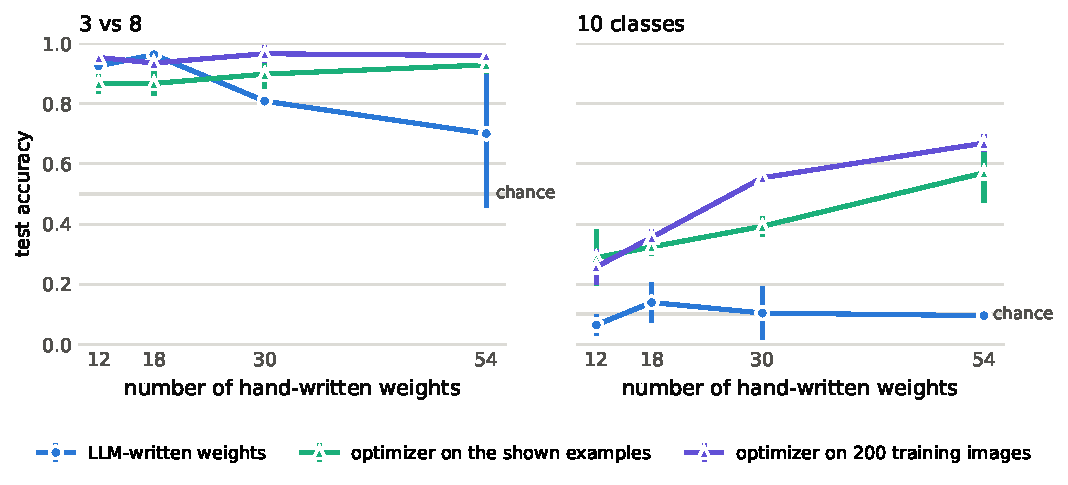
\includegraphics[width=\linewidth]{figures/scaling.pdf}
\caption{Scaling the fixed ansatz. Test accuracy against the number of hand-written weights (amplitude encoding + HEA with 1, 2, 4 and 8 layers) for the model, the optimizer on the shown examples, and the optimizer on 200 training images.}
\label{fig:scaling}
\end{figure}

Figure~\ref{fig:scaling} shows what happens as the circuit deepens. For 3 vs 8 the optimizer's accuracy rises monotonically with depth ($0.87 \to 0.93$ on the shown examples) while the model's falls: $0.81 \pm 0.02$ at 30 weights and $0.70 \pm 0.25$ at 54. For ten classes the circuit is too weak at 12--18 weights for anyone (the optimizer on the shown examples reaches $0.29$--$0.32$, and $0.26$--$0.36$ with 200 images), but with 30 and 54 weights it becomes a usable model for the optimizer ($0.39$ and $0.57$ on the shown examples; $0.55$ and $0.67$ with 200 images) and the model stays at chance throughout ($0.07$--$0.14$). Its replies at depth are candid: ``these are hand-designed heuristic weights, not optimized or validated weights''. Started from the model's 54 weights, the optimizer reaches $0.59$, so the weights are not harmful, merely uninformative.

\subsection{Cost}
A request cost on average 1.8k output tokens and 45 s for QAOA, 3.0k tokens and 160 s for VQE, and 5.2--5.5k tokens and 100--150 s for QML; the ten-class free-design circuits were the largest replies (14k tokens, 240 s). A single evaluation of the resulting circuit on our simulator takes milliseconds; the optimizer baselines took seconds to a minute per run.
